%%%%%%%%%%%%%%%%%%%%%%%%%%%%%%%%%%%%%%%%%
% Large Colored Title Article
% LaTeX Template
% Version 1.1 (25/11/12)
%
% This template has been downloaded from:
% http://www.LaTeXTemplates.com
%
% Original author:
% Frits Wenneker (http://www.howtotex.com)
%
% License:
% CC BY-NC-SA 3.0 (http://creativecommons.org/licenses/by-nc-sa/3.0/)
%
%%%%%%%%%%%%%%%%%%%%%%%%%%%%%%%%%%%%%%%%%

%----------------------------------------------------------------------------------------
%	PACKAGES AND OTHER DOCUMENT CONFIGURATIONS
%----------------------------------------------------------------------------------------

\documentclass[letterpaper]{article}	 % A4 paper and 11pt font size
\usepackage[english]{babel} % English language/hyphenation
\usepackage[protrusion=true,expansion=true]{microtype} % Better typography
\usepackage{amsmath,amsfonts,amsthm} % Math packages
\usepackage[svgnames]{xcolor} % Enabling colors by their 'svgnames'
\usepackage{booktabs} % Horizontal rules in tables
\usepackage[margin=1.0in]{geometry}
\usepackage{xcolor}
\usepackage{float}
\usepackage{alltt}
\usepackage{graphicx}
\usepackage{subcaption}
\usepackage{lastpage} % Used to determine the number of pages in the document (for "Page X of Total")

%----------------------------------------------------------------------------------------
%	TITLE SECTION
%----------------------------------------------------------------------------------------

%----------------------------------------------------------------------------------------

\begin{document}

\begin{center}
    \Large
    \textbf{Assignment 1: \\ Matrix Multiplication}
    
    \vspace{0.4cm}
    \large
        
    \vspace{0.4cm}
    Lara Backer \\ Unmukt Gupta \\ Edward Tremel

\end{center}

%----------------------------------------------------------------------------------------
%  CONTENTS
%----------------------------------------------------------------------------------------

\section{Overview}

Matrix multiplication is one of the most fundamental computations required to solve linear systems, and as such is of vital importance in numerous computational applications. Therefore, reducing computation time for matrix multiplication calculations is an obvious method for increasing the efficiency of many solvers. \\

In this paper, we will be discussing the implementation and results from multiple methods for optimizing matrix multiplication of equation \ref{eq:mm}, with matrix dimensions M, N, and K. Results are compared to often-used matrix multiplication routines, such as those present in BLAS, a basic blocked multiplication method, and a naive matrix multiplication routine. 

\begin{equation}
\text{C (M x N) = A (M x K) * B (K x N)}
\label{eq:mm}
\end{equation}

\section{Optimization Techniques}

\subsection{Blocking}
Blocking techniques take advantage of the temporal locality of inner loops. Each chunk, or 'block', of a matrix, is chosen so that the code loads the necessary block into cache for each loop, discarding the block when the loop is finished. Matrix multiplication is performed block by block. By knowing the cache level sizes, the block sizes can be chosen to fit within the cache and avoid cache misses, which will decrease code performance. \\ 

\noindent The head node on the totient cluster used to run this code is a Intel Xeon E5-2620 v3 processor. We first computed the cache sizes to try to figure out the optimal block sizes, as shown in the next subsections. 

\subsubsection{Level 1 Cache}
The processor level 1 cache size is 32KB. To fit both blocks for A and B, for a square matrix and double matrix values (8 bytes), the formula to compute the optimal desired block size is:

\begin{equation}
\text{2*(block size)$^2$*(double size) = cache size}
\end{equation}

\noindent Thus, the maximum size for this blocking and for square matrices is 44x44.

\subsubsection{Level 2 cache}
For the head node, the processor level 2 cache size is 256KB. At this point, two stages of blocking are performed, one for the level 1 cache (smaller blocks), and one for level 2 (larger blocks). \\ \\

Using the same formula as for the level 1 cache, the maximum size for the level 2 blocking is 126. \\ \\

We used the results from these starting calculations for block sizes, and tested block sizes in a range around them as well. 

\section{Index Order}
All index orders for loops in the smallest blocked matrix multiplication routine were tested. It was found that the default i,j,k ordering was optimal for the code and blocking, as it was written.

** Include graphs here, as possible**

\subsection{Copy Optimization}
Copy optimization improves spatial locality and reduces cache conflicts by copying fixed size blocks (row major for matrix A, column major for matrix B) and storing them elsewhere for the computation. Due to the additional data storage, it primarily optimizes code for large matrix computations. 

** Include graphs here as possible **

\subsection{SSE Directives}

Intel intrinsic functions were tested, in an attempt to use non-temporal storage instructions. Performance to specify non caching writes. We modified the dgemm\_basic as follows:

\begin{verbatim}
void basic_dgemm(const int lda, const int M, const int N, const int K,
                 const double* restrict A, const double* restrict B, double* restrict C)
{
    int i, j, k;
        __m128d atemp,btemp,ctemp,cij
    for (i = 0; i < M; ++i) {
        for (j = 0; j < N; ++j) {
            cij = _mm_load_sd(&C[j*lda+i]);
                for(k = 0;k<K;++k) {
                        atemp = _mm_load_sd(&A[k*lda+i]);
                        btemp = _mm_load_sd(&B[j*lda+k]);
                        ctemp = _mm_mul_sd(atemp,btemp);
                        cij = _mm_add_sd(cij,ctemp);
            }
            _mm_stream_pd(&C[j*lda+i],cij);
        }
    }
}
\end{verbatim}

\begin{figure}[H]
\centering
  \centering
  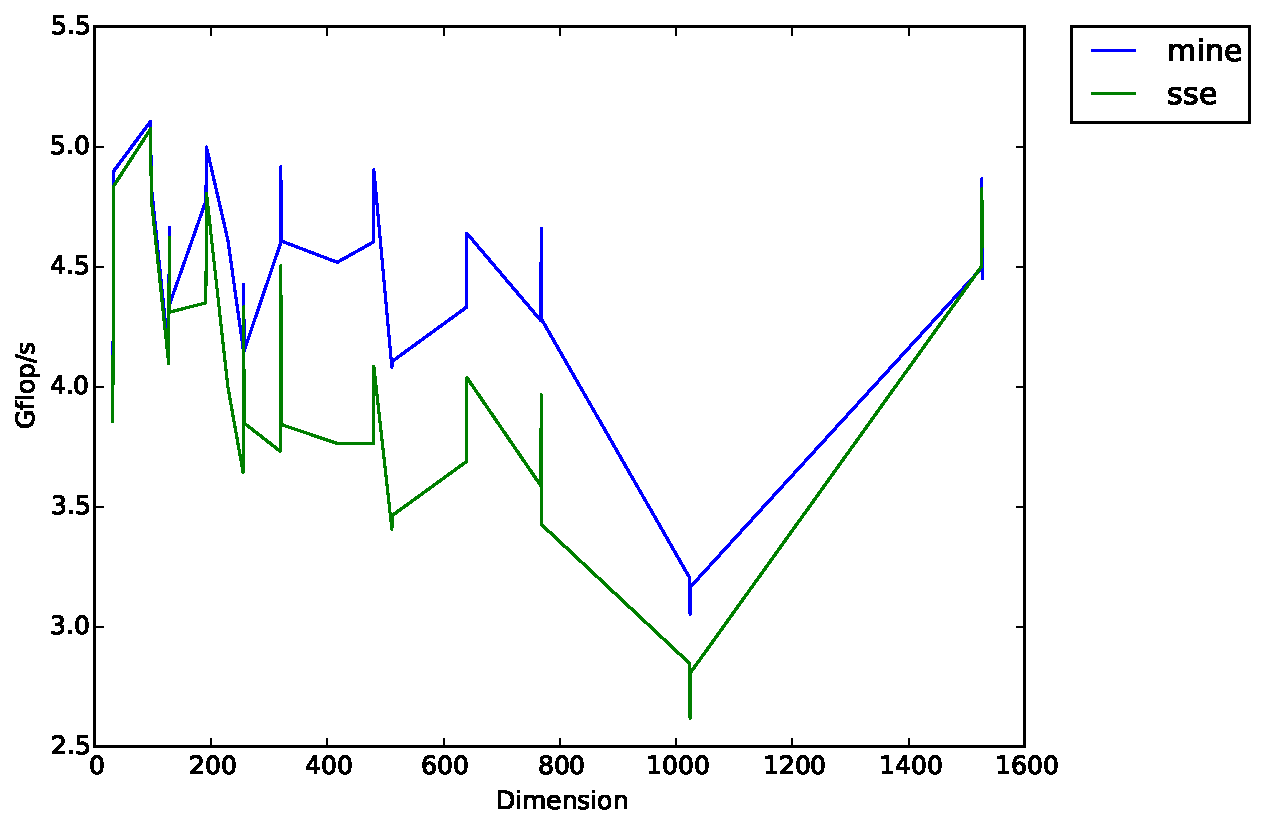
\includegraphics[width=.6\linewidth]{timing_sse.pdf}
  \caption{SSE Comparison Graph}
  \label{fig:sse}
  \end{figure}
  
  As can be seen in Figure \ref{fig:sse}, the timings for the modified SSE code were actually worse when compared to the basic blocked dgemm\_mine code. 


\subsection{Compiler Flags}
Compiler flags that were found to improve performance were for this code are listed as follows: \\
\begin{itemize}
\item -O2: Maximizes speed, enables vectorization. Basic optimize flag. 
\item -mfpmath=sse: Enables XMM registers in floating point operations
\item -Ofast: Enables high level aggressive optimizations -O3, -no-prec-div, and -fp-model fast=2. 
\\ 

Additional options were tested, such as -ipo, -flto, and -march=native. However, none of the flags were actually shown to increase efficiency. A comparison of the timings for options with all bulleted flags (flags), just the -O3 flag (o3), and no flags used (noflags) is shown in Figure \ref{fig:flags}. 

\begin{figure}[H]
\centering
  \centering
  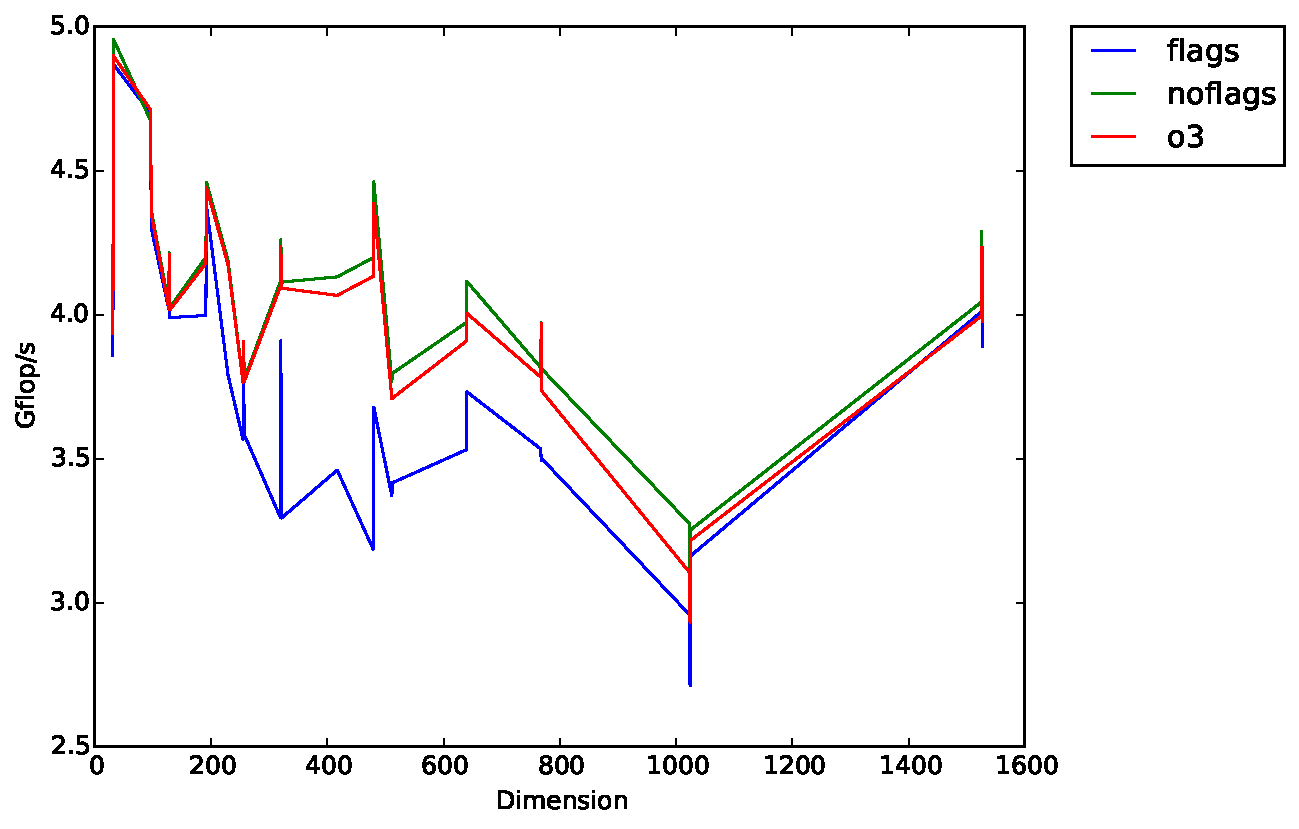
\includegraphics[width=.6\linewidth]{timing_flagcompare.pdf}
  \caption{Flag Comparison Graph}
  \label{fig:flags}
  \end{figure}

\end{itemize}

\section{Conclusion}

The final timing graphs for our code is shown in Figure XXX, compared to pre-written routines provided.

%----------------------------------------------------------------------------------------

\end{document}